\chapter{Background Theory}\label{chp:fundament}
%\vspace{-1.5cm}
%\noindent\rule{\columnwidth}{1.2mm}

\section{Robot operating system}

There are many problems when developing robot applications, especially because of the complexity of those systems. As more and more functionality is added to the robot, the code base becomes fluttered with intricate dependencies and entangled libraries. ROS (Robot Operating System) is not an operating system per se, but a framework that allows coders to readily develop and test solutions with modularity and code reusability in mind. It was built in an agnostic package system that allows integration with many packages available from the ROS Open-source community, a lot of them implementing support libraries and proof-of-concept algorithms, as well as core infrastructure.

The main aspects of ROS are \cite{quigley2009ros}:

\begin{itemize}
\item Peer-to-peer: even though the ROS framework relies on a master or namespace as a lookup mechanism, the communication is established between peers, avoiding unnecessary routing through slow links when the recipient is on the same subnet.
\item Tools-based: instead of building an intricate framework, ROS relies on a set of tools written to perform specific tasks, including various tools for compilation, tap data stream, data plotting, configuration, documentation generation, etc. Custom tools can even be written by the user in the form of new packages.
\item Multi-lingual: since communication between nodes relies only on XML-RPC, they can be implemented in any language, either by explicitly writing the full library that interacts with the ROS Core or building a wrapper for the ROS C++ library.
\item Thin: many robots implementations have parts of the code that could be reused in another project if they weren't so entangled with all existing code. ROS proposes an architecture where the code is separated into packages that hold no dependency on ROS. All packages can be built individually using CMake, different from the traditional software paradigm where one CMake file builds the entire project.
\item Free and Open-source: ROS source code is publicly available and released under the BSD License, allowing you to copy, modify and redistribute the source code, including for commercial purposes.
\end{itemize}

The execution of ROS is separated into smaller pieces of code that do particular tasks, called nodes. Each time ROS Core is launched, a collection nodes that are required for execution are spawned: the ROS master, that provides support for the registration of all subsequent nodes, the ROS parameter server, to register parameters during execution time, and the \texttt{rosout} node, for logging purposes. Once the core is launched, every other node can be spawned.

\subsection{Packages}

In order to better build robotic systems, ROS adopts a packaged architecture, making every subsystem of the application separate from all the others. Every package can contain new nodes, libraries, configuration or even datasets.

The main advantage of this approach is making the code more organized in its own subsystems, that specialize in doing a specific task well so that other packages can use this functionality. Packages can also be written independently of language, as long as it's supported by ROS.

\subsection{Topics}

In order for nodes to communicate, they interact by publishing messages in topics. Topics are anonymous buses where each node can publish messages following the message type standards. Each node can then subscribe to topics that are relevant to them and act upon data captured on the topic. Message can even be recorded and played back to support applications that will need the information later in time.

% TODO: refazer imagem para evitar citação
\begin{figure}[!ht]
\centering
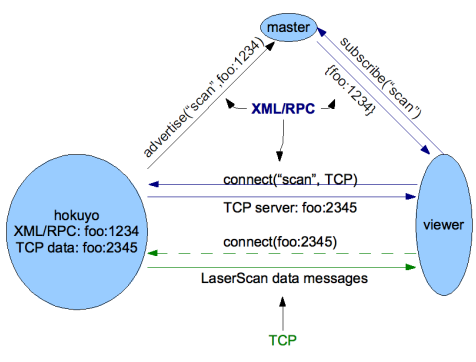
\includegraphics[width=0.66\linewidth]{rostopic}
\caption[Topic initialization.]{Topic initialization \cite{rosoverview}.}
\label{fig:rostopic}
%\small{Source: ROSWiki.}
\end{figure}

The topics are implemented in the XML-RPC protocol, using a master node in order to provide name resolution. In order for a publisher to connect to a subscriber, they do the following steps \cite{rosoverview}:

\begin{enumerate}
\item Subscriber register with the master the topics it will be listening to.
\item Publisher register with the master the topics it will be publishing to.
\item Master informs the subscriber of a new publisher.
\item Subscriber requests a topic connection with the Publisher and negotiates a transport protocol.
\item Subscriber connects using the selected protocol.
\end{enumerate}

The process described above is illustrated in \prettyref{fig:rostopic}. It's important to notice that, once the connection is established, the communication is maintained peer-to-peer, using former protocols like TCPROS, built over TCP, and UDPROS, built over UDP. This not only provides faster communication inside the same network by not requiring the messages to be relayed through the master but also enables communication through available networks of the Internet protocol suite, including 802.11X wireless transmission.

The topic configuration also enables true agnostic packages, since the communication between them will be done using a standardized communication medium, loosely coupling the packages and making them easily maintainable. Debugging can also be done using command-line tools that wiretap this medium and display the information exchanged by nodes.

\subsection{Services}

The topic communication can be very useful in many-to-many communication but lacks support when sending messages or commands that require a response. When a reply is needed, it is a better practice to use services instead of topics. This is especially true for tasks that need a lot of computing power but only need to be executed once in a while, so instead of calculating it in every iteration, the service can be run just when requested and return data to the caller. The request is usually done in a similar way to Remote Procedure Calls (RPCs) in programming languages.

\subsection{Message types}

Since nodes need to understand each other, they talk following pre-defined message standards, and the message files themselves are packages that define the content of each message. To avoid confusion, each topic is initialized using a pre-defined message type and every node has to conform to it. Let's take a look at the message definition \texttt{geometry\_msgs/Twist.msg}, that is used in navigation to define linear and angular velocity for the joints:

\begin{lstlisting}
Vector3  linear
Vector3  angular
\end{lstlisting}

Note that the \texttt{Vector3} is not a base type message, but is another type of message defined at \texttt{geometry\_msgs/Vector3.msg}:

\begin{lstlisting}
float64 x
float64 y
float64 z
\end{lstlisting}

The variable types that cannot be expanded into other definitions are called primitive types. The primitive types are:

\begin{multicols}{3}
    \begin{itemize}
        \item \texttt{bool}
        \item \texttt{int8}
        \item \texttt{uint8}
        \item \texttt{int16}
        \item \texttt{uint16}
        \item \texttt{int32}
        \item \texttt{uint32}
        \item \texttt{int64}
        \item \texttt{uint64}
        \item \texttt{float32}
        \item \texttt{float64}
        \item \texttt{string}
        \item \texttt{time}
        \item \texttt{duration}
    \end{itemize}
\end{multicols}

Message types for services are done in a similar way, but since services support response, the message will consist of two individual messages. If we look at a standard definition found in \texttt{std\_srvs/SetBool.srv}:

\begin{lstlisting}
bool data
---
bool success
string message
\end{lstlisting}

This service is used for setting a boolean variable to \textit{true} or \textit{false}, that can be activating or deactivating an actuator. The response consists of a boolean that tells if the operation was successful and a message for better description in case of error.

\section{Transformations}

Transformations, or tfs, for short, are the way ROS deals with coordinates frames in space. As the poses for each link in the robot might change over time, it keeps track of these changes and provides tools to assist the user to do transformations with the data.

Suppose a particular robot has a reference fixed frame \texttt{/world} in the origin. The center of the robot is another frame called \texttt{base\_link}. The transformation \texttt{/world -> /base\_link} would indicate the position of the robot relative to the world.

Now, let's say the robot has a laser scanner sensor \texttt{/laser\_link} relative to \texttt{/base\_link}, as it is fixed on the robot. The laser makes a measurement and this result is relative to the laser position. Let's call the result \texttt{/result}. The result is then related to \texttt{/world} by a long chain of transformations.

\begin{verbatim}
/world -> /base_link -> /laser_link -> /result
\end{verbatim}

It can be tricky to transform the \texttt{/result} back to \texttt{/world} coordinates. The tf package gives the user an easy way of setting up a listener on the \texttt{/tf} topic that will listen to the published transforms and do the required transformations between coordinate frames, so the user can ask directly for the transform \texttt{/world -> result} instead of transforming the data himself.

\section{Simulation}

Since deploying a test robot at every code change is costly and time consuming and ROS only provides the tools to develop a robot system solution, there is a need for offline simulation of the robots, avoiding having to test every configuration on physical hardware. In these cases, it can be helpful to set up a rigid body simulation. The normal workflow for setting up a simulation is \cite{russell2004}:

% http://ode.org/slides/slide2.html
\begin{itemize}
    \item Isolating the important variables in the physical process.
    \item Model the physical system behavior using equations.
    \item Find a method to solve the equations, given the inputs and the initial state of the system.
    \item Write a computer program that can do that simulation.
    \item Simulate and benchmark the results against the physical system.
\end{itemize}

Repeating all these five steps for every physical system will lead to the best results, but can be time-consuming and difficult because all the variables involved. Since the possibilities for a robot system are often limited, physics engines or physics SDKs (source development kits) were developed to aid simulation.

While the real world has a lot of complexity, rigid body dynamics can be simplified in rigid bodies, joints, collisions, friction and springs, elements that are important to the process. The physical model can be reduced to the laws of motion, using mass, velocity, acceleration, and force as simulation variables. Since the model and the solution to these problems are well known, generalized solvers can be written that compute the simulation at each instant of time, or time steps.

Many simulators implement this generalized solvers, as well as render the 3D models to show to the user, including game engines like Unity and USARSim (based on Unreal engine), commercial solutions like Microsoft Robot Studio, Webots and MATLAB, and open-source projects like Gazebo \cite{craighead2007survey}. Since Gazebo adopts the mentality of the ROS project of being open and free, it became widely used in the community, and as a result better developed over time.

Gazebo provides ROS with a framework to simulate and benchmark the robot or even a group of robots accurately. \prettyref{fig:gazebo-sim} shows the Gazebo simulation for a supported robot \cite{koenig2004design}.

\begin{figure}[!ht]
\centering
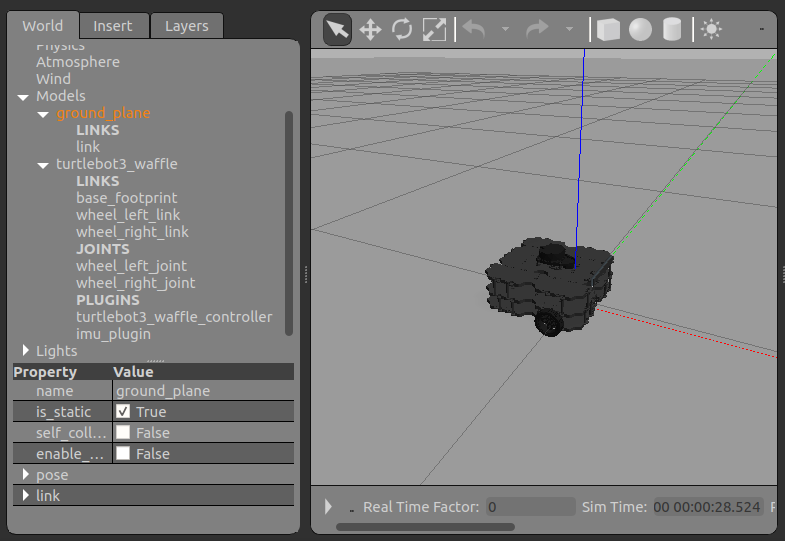
\includegraphics[width=.5\linewidth]{gazebo-sim}
\caption{Gazebo simulation suite.}
\label{fig:gazebo-sim}
\end{figure}

The Gazebo simulator offers:

\begin{itemize}
\item Dynamics simulation using multiple physics engines.
\item Advanced 3D graphics for high-quality rendering.
\item Sensors and noise, to generate reliable sensor data, compatible with real-world sensors.
\item Robot models, including ones from the community.
\end{itemize}

All the robot description is made using a URDF (Universal Robotic Description Format) file or an SDF (Simulation Description Format) file. The URDF  file is an XML file describing all elements of the robot. Even though it's called ``Universal'', it lacks some of the features like parallel linkages, friction, etc. To get around these issues, a new model called SDF was developed specifically for use in Gazebo, while the URDF was maintained for backward compatibility. Every time a URDF file is loaded, it is converted by Gazebo to an SDF equivalent.

\subsection{URDF}

URDF files starts describing each link of the robot and it's respective inertia. \prettyref{fig:gazebo-sim} show an example of the robot Turtlebot3 Waffle \cite{turtlebot3} consisting of three links: \texttt{base\_footprint}, \texttt{wheel\_left\_link} and \texttt{wheel\_right\_link}. They are loaded from STL or Collada files included in the project. \prettyref{fig:gazebo-stl} show the STL renders for the robot shown on \prettyref{fig:gazebo-sim}.

\begin{figure}[!ht]
\centering
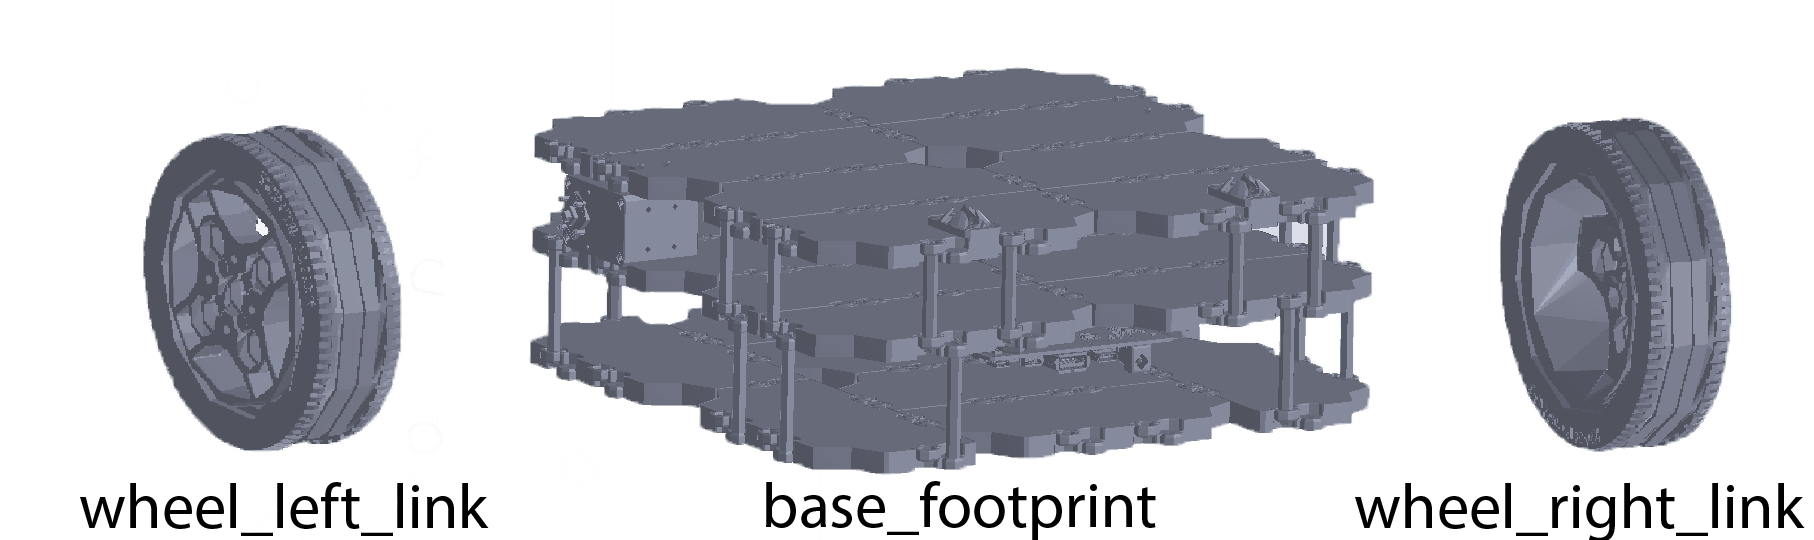
\includegraphics[width=.8\linewidth]{gazebo-stl}
\caption{STL Link files.}
\label{fig:gazebo-stl}
\end{figure}

The inertia is described by its inertial parameters, namely the mass, center of mass and moment of inertia matrix. Additionally, collision box that will aid collision testing in simulation can be specified. The user can then describe the rest of the robot, including the joints that will hold links together. Two basic joints can be seen, \texttt{wheel\_left\_joint} and \texttt{wheel\_right\_joint}, that hold all three links together. Finally, the plugins will give the robot the simulation functionality, adding IMUs, Laser Scanners, Cameras, etc.

\subsection{SDF}

The SDF is an improvement of the URDF descriptor format that supports more functionality. It not only supports all the physical descriptions shown in the URDF model but also features:

\begin{itemize}
\item World information, from lightning and gravity to complex information like magnetic fields, winds, and atmosphere (temperature and pressure).
\item Scene information, like ambient, background, sky, fog and shadows.
\item Multiple robots descriptors.
\item Choosing a physics engine.
\end{itemize}

\subsection{Physics engines}

In order to simulate the physical conditions of the robot and the environment, Gazebo supports four different physics engines: ODE, Bullet, Simbody, and DART. At the start of each simulation, the user can select the desired physics engine changing the startup flags for the program, or configure it on the SDF file.

ODE or Open Dynamics Engine is an engine for simulating articulated rigid body structures. It features a stable integrator, meaning that numeric errors may not grow out of control. Because of that, the simulator drops physical accuracy in favor of speed, stability and robustness \cite{smith2005open}.

Bullet is a Python implementation of physics simulation for robotics, games, and visual effects that provides forward and inverse dynamics and kinematics, as well as built-in collision detection. Bullet differentiates itself by being easy to use and provides integration to machine learning frameworks like TensorFlow \cite{coumans2018}.

Simbody is a multibody simulator focused on biomedical research. It was developed to better suit simulation scenarios where engines like ODE may not converge to correct results due to its lack of fidelity. It is used for neuromuscular, prosthetic, and biomolecular simulation, as well as design and control of humanoid robots \cite{sherman2011simbody}.

DART or Dynamic Animation and Robotics Toolkit is another rigid body simulation that distinguishes itself due to its accuracy and stability. The main purpose of this simulator is to provide full access to internal kinematic and dynamic quantities \cite{lee2018dart}.

All four engines are used to tackle different problems. By varying the time step, for instance, you might obtain better results in your simulation with one of the engines. Usually, when choosing the simulation engine, the relationship between the number of iterations, error, and speed must be taken into account. Some of the simulations require greater precision, while others may require real-time performance. For a more in-depth comparison of the four engines see \cite{peters2014comparison}.

\subsection{Sensors and actuators}

Gazebo also allows simulating sensors and actuators that will interact with the world and send data back to ROS packages. Sensors can include cameras, laser scanners, contact sensors, IMU, RFID, Sonar, Magnetometer. Actuators can use the ROS control library to actuate joints. The sensors are described in the SDF or URDF files. The example below shows an example of a camera description.

\begin{lstlisting}[caption=Exemple of a URDF file for a camera description., language=XML]
  <gazebo reference="camera_link">
    <sensor type="camera" name="camera1">
      <update_rate>30.0</update_rate>
      <camera name="head">
        <horizontal_fov>1.3962634</horizontal_fov>
        <image>
          <width>800</width>
          <height>800</height>
          <format>R8G8B8</format>
        </image>
        ...
      </camera>
      <plugin name="camera_controller" filename="libgazebo_ros_camera.so">
        <alwaysOn>true</alwaysOn>
        <updateRate>0.0</updateRate>
        <cameraName>robot/cam1</cameraName>
        <imageTopicName>image_raw</imageTopicName>
        <cameraInfoTopicName>camera_info</cameraInfoTopicName>
        <frameName>camera_link</frameName>
        <hackBaseline>0.07</hackBaseline>
        <distortionK1>0.0</distortionK1>
        <distortionK2>0.0</distortionK2>
        <distortionK3>0.0</distortionK3>
        <distortionT1>0.0</distortionT1>
        <distortionT2>0.0</distortionT2>
      </plugin>
    </sensor>
  </gazebo>
\end{lstlisting}

The controller is loaded from a plugin called \texttt{libgazebo\_ros\_camera.so} and uses as parameters which topic the camera will correspond to and the intrinsic parameters of the lenses, update rate and sensor type, as well as the link the camera will be attached to.

There are many pre-built plugins available at Gazebo library, including Cameras (mono and stereo), Kinect, Laser Scanner, Force and IMU sensors, Differential Drive, Skid Steering Drive, as well as templates to write your own dedicated plugin.

%\section{OpenCV}

%\section{MoveIt}

%MoveIt is a ROS library aimed at simplifying motion planning for complex robots. It is the evolution of \texttt{arm\_navigation} package, designed for motion planning, trajectory generation and environment monitoring for the PR2 robot \cite{chitta2012moveit}.

%One of the main requirements of robots working closely to humans and the dynamic environment is that they can detect and avoid collisions and other obstacles efficiently. MoveIt does this by creating a probabilistic 3D model of the environment using Octomaps. This is important because physical sensors have noise and inaccuracies, and the Octree representation is also much more efficient.

%With a model in hand, MoveIt can make use one of the available planners: Open Motion Planning Library (OMPL), Stochastic Trajectory Optimization for Motion Planning (STOMP), Search-Based Planning Library (SBPL), and Covariant Hamiltonian Optimization for Motion Planning (CHOMP). Having different planners available is important because they allow different movement constraints. One trajectory might need the manipulator to be always upright, like carrying liquids, while other doesn't have this constraints. MoveIt uses a configuration wizard to generate configuration files based on the URDF or SRDF robot model, making the package robot agnostic. In the configuration, the user can specify the attributes desired for the robot.

%The Self-collisions options allow you to select the density of the Self-collision matrix. Higher densities require more computation whereas lower densities might disable valid options. Virtual joints allows you to define which joints attach the robot to the world frame. Planning groups are used to virtually separate distinct parts of the robot, that may include creating joint groups on what composes the left arm, right arm, manipulator, etc. Robot poses defines fixed poses as reference for the robot, that may include \textit{Home} or \textit{Resting} positions. The End-effectors configuration is used to further specify which of the planning groups are end effectors, that may include tools and grippers. Finally, the passive joints configuration is used to specify the joints that cannot be actuated on, and thus cannot be used for motion planning.

%There are also plugins for RVIZ visualization of the planned trajectories. They help by providing visual tools to work with the robot, examining poses and testing trajectories behavior. There are also many plugins available for Inverse Kinematics calculation, as well as wrappers to write your own solver.

\section{Care-o-bot}

Care-o-bot is a project for a mobile assistive robot that is modular, developed and maintained by Fraunhofer IPA. COB's fourth version, \prettyref{fig:cob4}, was designed not only to provide researchers a reliable mobile base, but also to aid research on human-robot interaction and social behavior \cite{mci/Kittmann2015}. It is composed mainly by a mobile base, a torso, and a head.

% TODO: editar a imagem para conter descrição de partes
\begin{figure}[!ht]
\centering
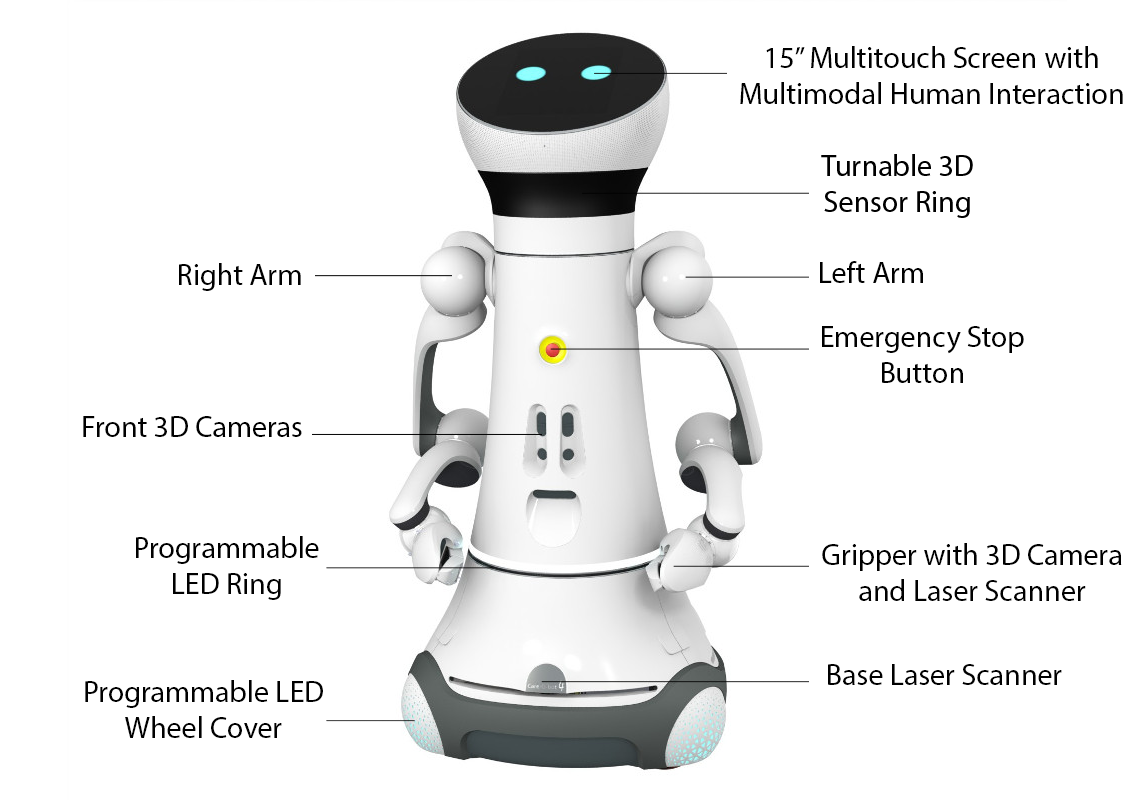
\includegraphics[width=.8\linewidth]{cob4}
\caption[COB 4 full robot with both manipulators.]{COB 4 full robot with both manipulators \cite{care-o-bot-image-full}.}
\label{fig:cob4}
\end{figure}

\subsection{Base}

The base features three steerable wheels used for moving the robot on the ground. Because the modularity, the wheels can be configured to use Ackermann kinematics, moving forward and backward and rotating on the vertical axis, but also Omnidirectional kinematics, allowing the robot to move in every direction. The maximum speed supported is 1,1 m/s. It is also equipped with three 2D laser scanners with 360$^{\circ}$ coverage for object detection and safety, and the battery pack to power the robot and the control panel.

\subsection{Torso}

The torso is linked with the base, and can be configured to be fixed (the torso doesn't move), to use a Pan joint (allowing for a full rotation) or using a spherical joint (providing 3DOF). It can have two optional arms with 7DOF, each with a robotic hand with two fingers (2 DOF hand). The torso also features 3D cameras on the front and in the back.

\subsection{Arms}

Arms are composed of three SCHUNK Powerball ERB modules and one PRL+ 100 module, a rotary actuator, in the shoulder. The arm is a variation of the commercially available Schunk arm called LWA4P, which has 6 DOF and is composed of three Powerball ERB, with 2 DOF each. The last degree of freedom is provided by the PRL+, allowing one rotation around the shoulder and totaling 7 DOF. \prettyref{fig:schunk_lwa4p_extended} shows the full arm in simulation. The manipulator's finger was developed by Schunk specifically for this robot.

The manipulator also has a 3D camera and laser pointer for object recognition and picking, as well as LEDs for illumination. The torso also provides 3D cameras and sensors for computer vision activities that cover up the front of the robot and an LED Ring for signaling and an emergency stop.

\begin{figure}[!ht]
    \centering
    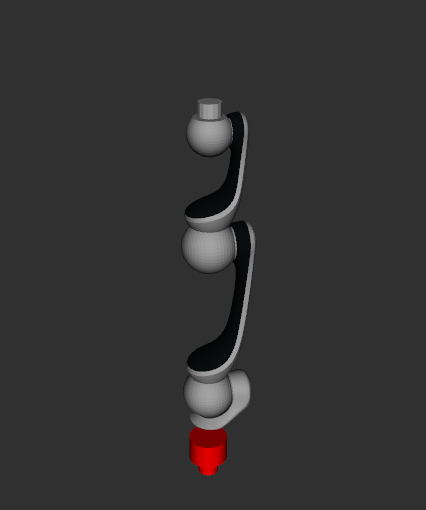
\includegraphics[width=.3\linewidth]{schunk_lwa4p_extended}
    \caption{LWA4P extended arm.}
    \label{fig:schunk_lwa4p_extended}
\end{figure}

The LWA4P arm was designed to operate at low power at battery-dependent devices and is capable of lifting a maximum payload of 6kg. Each joint in the Powerball is capable of rotating to $\pm 170^\circ$, at a maximum speed of $72^\circ /\text{s}$, and the overall repeat accuracy of the arm is $\pm 0.15 \ \text{mm}$.


\subsection{Head}

The head is linked with the torso, allowing for both a pan joint or a spherical joint, and contain the human interface to interact with the user, including the sound system, microphone, a touch screen display and optional camera for face recognition.


\subsection{Package organization}

COB is built around ROS and combines different sets of packages for different purposes. Since the robot support different configurations (manipulators, joints, mobile bases), some packages are optional. \prettyref{fig:dependency-graph} shows the dependency graph for the first three layers of packages. Notice that the arrangement is quite intricate even showing only the packages written exclusively for COB (not showing other ROS packages used on COB).

\begin{figure}[!ht]
\centering
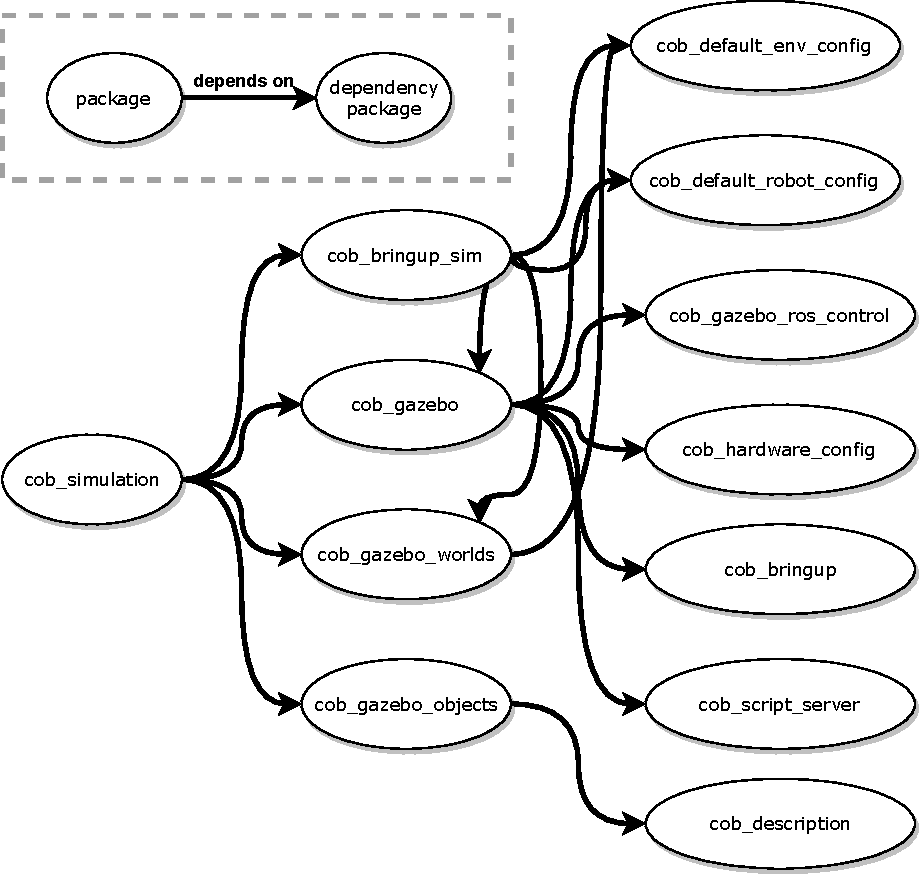
\includegraphics[width=.7\linewidth]{dependency-graph}
\caption{Dependency graph of \texttt{cob\_simulation} with depth 3.}
\label{fig:dependency-graph}
\end{figure}


The COB core consist of the following packages and its dependencies:

\begin{itemize}
\item \texttt{cob\_msgs}: Robot-specific Messages, representing state information like battery status, etc.
\item \texttt{cob\_srvs}: Robot-specific Services.
\item \texttt{cob\_description}: Robot URDF models for different COB configurations (only base, base with fixed torso, base with actuated torso, etc).
\item \texttt{cob\_bringup}: machine configuration, including all scripts and dependencies required to run COB, both in simulation and real hardware.
\end{itemize}

COB also features high-level capabilities, some of them being:

\begin{itemize}
\item \texttt{cob\_command\_tools}: high-level utilities command tools, including API for commonly used movements, control dashboard, teleoperation and status monitoring.
\item \texttt{cob\_driver}: plugins interfacing motors, LEDs, sound system, cameras, batteries and even the facial expressions for the robot, and providing their data in the form of topics and services.
\item \texttt{cob\_navigation}: provides tools for robot navigation, including creation of maps, navigation with/without collision avoidance and navigation in dynamic environments.
\item \texttt{cob\_object\_perception}, \texttt{cob\_people\_perception}, \texttt{cob\_environment\_perception}: computer vision libraries used for perception of the environment.
\item \texttt{cob\_manipulation}: manipulator related package, including inverse kinematics, arm motion planning and collision avoidance.
\end{itemize}

\subsection{Basic API}

Most of the capabilities of COB are exposed in the form of topics and services, forming a higher level API and sparing the user from interacting with low-level sensors and actuators.

The actuators move the three wheels on the base. Since the base kinematics is already calculated by the node, you only need to publish a \texttt{geometry\_msgs/Twist} type message with linear and angular velocities and the drivers will take care of the rest. The topic names can be seen on \prettyref{tab:baseapi}.

\begin{table}[!ht]
\caption{Base command API.} \label{tab:baseapi}
\renewcommand*{\arraystretch}{1.1}
\resizebox{\textwidth}{!}{
\begin{tabular}{c|c|c}
Topic Name & Message Type & Information \\
\hline
\makecell{\texttt{/base/twist\_mux} \\ \texttt{/command\_navigation}} & \texttt{geometry\_msgs/Twist} & Velocity topics related to navigation \\ \hline
\makecell{\texttt{/base/twist\_mux} \\ \texttt{/command\_safe}} & \texttt{geometry\_msgs/Twist} & \makecell{Velocity topics related to teleoperation \\ with collision checking and smoothing} \\ \hline
\makecell{\texttt{/base/twist\_controller} \\ \texttt{/command}} & \texttt{geometry\_msgs/Twist} & \makecell{Low level Velocity topics \\ for control purposes} \\ \hline
\end{tabular}
}
\end{table}

Since the torso and the head only have one joint, they receive a set of points forming a trajectory to follow, given by the \texttt{control\_msgs/FollowJointTrajectory} service message type. This service returns if the robot was able to perform the trajectory, as well as the error in the path. The structure can be seen on \prettyref{tab:headapi}.

\begin{table}[!ht]
\caption{Torso and head command API.} \label{tab:headapi}
\renewcommand*{\arraystretch}{1.1}
\resizebox{\textwidth}{!}{
\begin{tabular}{c|c|c}
Topic Name & Message Type & Information \\
\hline
\makecell{\texttt{/torso/joint\_trajectory\_controller} \\ \texttt{/follow\_joint\_trajectory}} & \texttt{control\_msgs/FollowJointTrajectory} & Trajectory to move the torso \\ \hline
\makecell{\texttt{/head/joint\_trajectory\_controller} \\ \texttt{/follow\_joint\_trajectory}} & \texttt{control\_msgs/FollowJointTrajectory} & Trajectory to move the head \\ \hline
\end{tabular}
}
\end{table}

The arms, the grippers and the sensor ring are similar to the torso and head, as they act as a service and receive the same message type. Their API is shown on \prettyref{tab:armapi}.

\begin{table}[!ht]
\caption{Arms and grippers command API.} \label{tab:armapi}
\renewcommand*{\arraystretch}{1.1}
\resizebox{\textwidth}{!}{
\begin{tabular}{c|c|c}
Topic Name & Message Type & Information \\
\hline
\makecell{\texttt{/arm\_left/joint\_trajectory\_controller} \\ \texttt{/follow\_joint\_trajectory}} & \texttt{control\_msgs/FollowJointTrajectory} & Trajectory to move the left arm \\ \hline
\makecell{\texttt{/gripper\_left} \\ \texttt{/joint\_trajectory\_controller} \\ \texttt{/follow\_joint\_trajectory}} & \texttt{control\_msgs/FollowJointTrajectory} & Trajectory to move the left gripper \\ \hline
\makecell{\texttt{/arm\_right/joint\_trajectory\_controller} \\ \texttt{/follow\_joint\_trajectory}} & \texttt{control\_msgs/FollowJointTrajectory} & Trajectory to move the right arm \\ \hline
\makecell{\texttt{/gripper\_right} \\ \texttt{/joint\_trajectory\_controller} \\ \texttt{/follow\_joint\_trajectory}} & \texttt{control\_msgs/FollowJointTrajectory} & Trajectory to move the right gripper \\ \hline
\makecell{\texttt{/sensorring} \\ \texttt{/joint\_trajectory\_controller} \\ \texttt{/follow\_joint\_trajectory}} & \texttt{control\_msgs/FollowJointTrajectory} & Trajectory to move the sensor ring ring\\ \hline
\end{tabular}
}
\end{table}

For the sensors, there are three lasers scans that cover the entire circumference of the robot, shown on \prettyref{tab:laserapi}. Even though they are separate entities, there are nodes that transform the three different measurements into a single one for easier use later on.

\begin{table}[!ht]
\caption{Laser Scan API.} \label{tab:laserapi}
\centering
\renewcommand*{\arraystretch}{1.1}
\begin{tabular}{c|c|c}
Topic Name & Message Type & Information \\
\hline
\texttt{/base\_laser\_front/scan} & \texttt{sensor\_msgs/LaserScan} & Front laser scan \\ \hline
\texttt{/base\_laser\_left/scan} & \texttt{sensor\_msgs/LaserScan} & Left laser scan \\ \hline
\texttt{/base\_laser\_right/scan} & \texttt{sensor\_msgs/LaserScan} & Right laser scan \\ \hline
\texttt{/scan\_unified} & \texttt{sensor\_msgs/LaserScan} & Unified laser scan \\ \hline
\end{tabular}
\end{table}

There are also cameras in the torso, head and in the sensor ring that collect both raw images and a point cloud representation that includes the distance of each point to the focal point of the camera. Their respective topics can be seen on \prettyref{tab:cameraapi}.

\begin{table}[!ht]
\caption{Cameras API.} \label{tab:cameraapi}
\renewcommand*{\arraystretch}{1.1}
\resizebox{\textwidth}{!}{
\begin{tabular}{c|c|c}
Topic Name & Message Type & Information \\
\hline
\texttt{/torso\_cam3d\_left/rgb/image\_raw} & \texttt{sensor\_msgs/Image} & \makecell{Color image of the \\ left torso camera} \\ \hline
\texttt{/torso\_cam3d\_left/depth\_registered/points} & \texttt{sensor\_msgs/PointCloud2} & \makecell{Depth data from \\ torso left camera} \\ \hline % left camera
\texttt{/torso\_cam3d\_right/rgb/image\_raw} & \texttt{sensor\_msgs/Image} & \makecell{Color image of the \\ right torso camera} \\ \hline
\texttt{/torso\_cam3d\_right/depth\_registered/points} & \texttt{sensor\_msgs/PointCloud2} & \makecell{Depth data from \\ torso right camera} \\ \hline % right camera
\texttt{/torso\_cam3d\_right/rgb/image\_raw} & \texttt{sensor\_msgs/Image} & \makecell{Color image of the \\ down torso camera} \\ \hline
\texttt{/torso\_cam3d\_down/depth\_registered/points} & \texttt{sensor\_msgs/PointCloud2} & \makecell{Depth data from \\ torso down camera} \\ \hline % down camera
\texttt{/sensorring\_cam3d\_front/depth/points} & \texttt{sensor\_msgs/PointCloud2} & \makecell{Depth data from \\ sensor ring camera} \\ \hline
\texttt{/sensorring\_cam3d\_back/rgb/image\_raw} & \texttt{sensor\_msgs/Image} & \makecell{Color image of the \\ back sensor ring camera} \\ \hline
\texttt{/torso\_cam3d\_down/depth\_registered/points} & \texttt{sensor\_msgs/PointCloud2} & \makecell{Depth data from \\ back sensor ring camera} \\ \hline % sensor ring back camera
\texttt{/head\_cam3d/rgb/image\_raw} & \texttt{sensor\_msgs/Image} & \makecell{Color image of the \\ head camera} \\ \hline % head camera
\end{tabular}
}
\end{table}

Finally, there are also other miscellaneous topics to control the lights and text-to-speak output and publish robot information, shown on \prettyref{tab:miscapi}.

\begin{table}[!ht]
\caption{Miscellaneous API.} \label{tab:miscapi}
\centering
\renewcommand*{\arraystretch}{1.1}
\resizebox{\textwidth}{!}{
\begin{tabular}{c|c|c}
Topic Name & Message Type & Information \\
\hline
\texttt{/joy} & \texttt{sensor\_msgs/Joy} & Input commands of joystick \\ \hline
\texttt{/sound/say} & \texttt{cob\_sound/Say} & Text for text-to-speak output \\ \hline
\texttt{/light\_base/set\_light} & \texttt{cob\_light/SetLightMode} & Command for base lights \\ \hline
\texttt{/light\_torso/set\_light} & \texttt{cob\_light/SetLightMode} & Command for torso lights \\ \hline
\texttt{/light\_torso/set\_light} & \texttt{cob\_light/SetLightMode} & Command for torso lights \\ \hline
\texttt{/emergency\_stop\_state} & \texttt{cob\_msgs/EmergencyStopState} & \makecell{Laser and button \\ stop information.} \\ \hline
\texttt{/power\_state} & \texttt{cob\_msgs/PowerState} & \makecell{Battery information.} \\ \hline
\end{tabular}
}
\end{table}